\subsection{Fusion Report}

\subsubsection{Fusion Techniques}
Considering that both Object A and Background Scene generate \textbf{point cloud},both Object Bs and Object Cs generate \textbf{mesh}, we export the point cloud as \textbf{gaussian mesh} with the code offered by 2DGS chapter and put all the resources into the Blender.

\subsubsection{Fusion Visualization}
Figure~\ref{fig:Fusion Vis} are some pictures of our fusion results, some include all objects, while some pick one from each category:

\begin{figure}[h]
	\centering
	
	% 第一行：full_1 和 full_2 并排
	\begin{minipage}{0.45\textwidth}
		\centering
		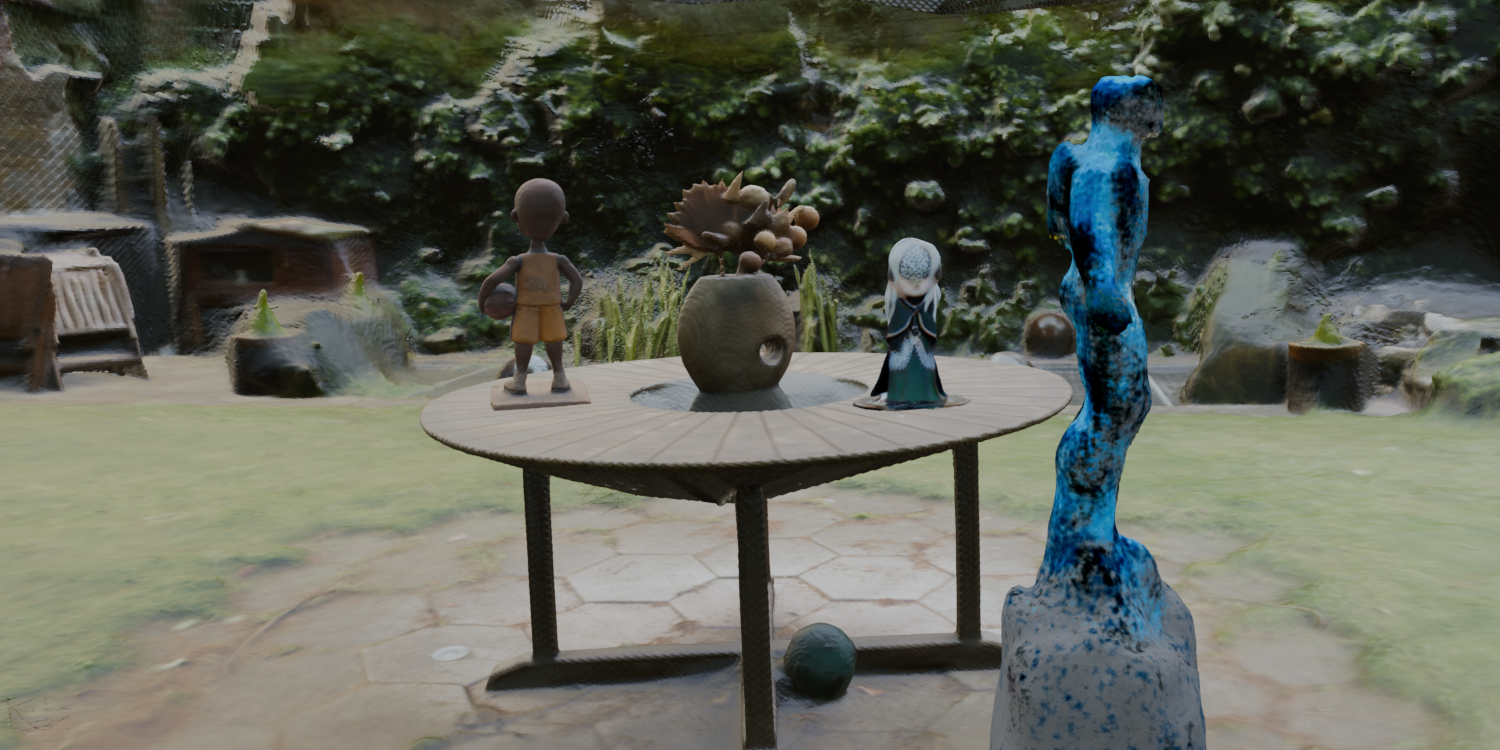
\includegraphics[width=\linewidth]{figures/task1/full_1.png}
	\end{minipage}
	\hfill
	\begin{minipage}{0.45\textwidth}
		\centering
		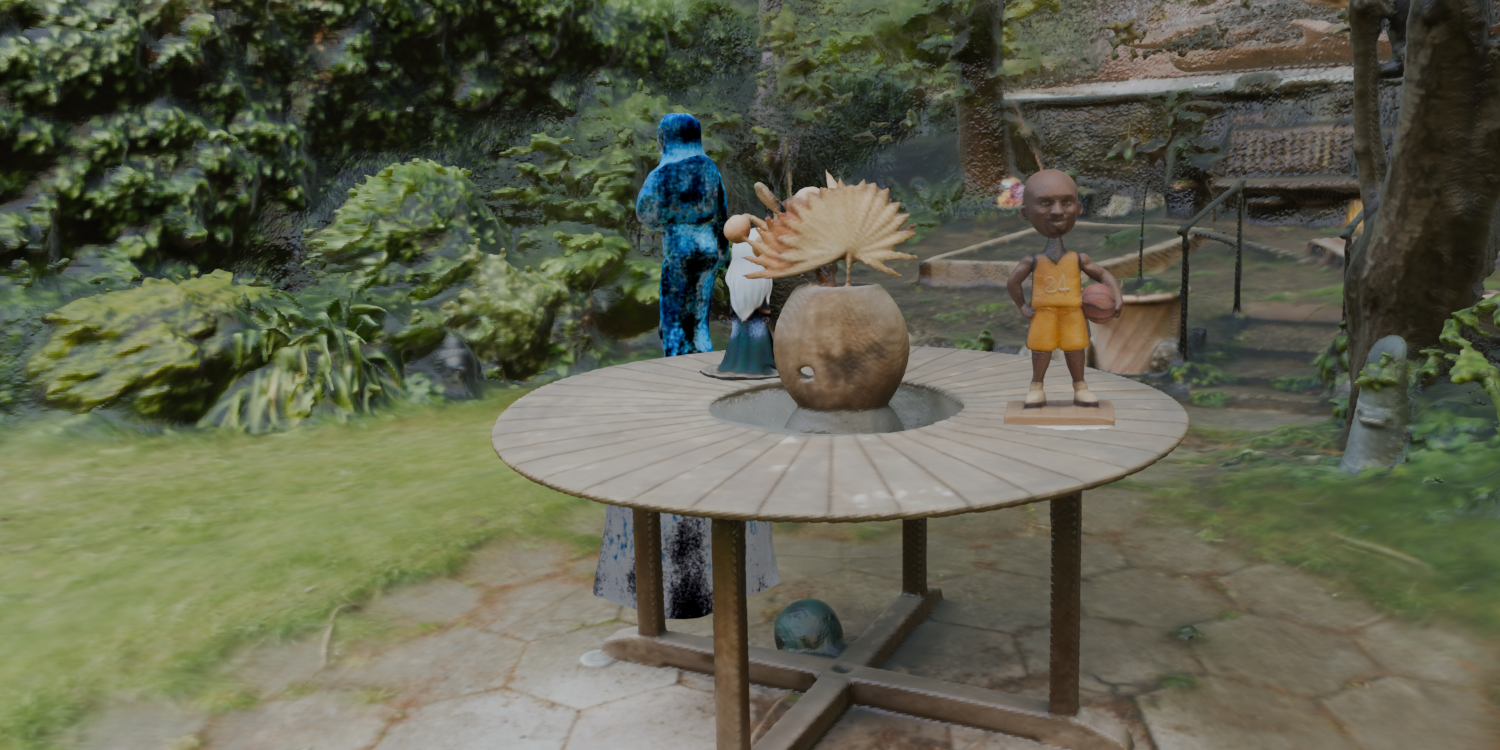
\includegraphics[width=\linewidth]{figures/task1/full_2.png}
	\end{minipage}
	
	\vspace{0.3cm}  % 行间距（可调整）
	
	% 第二行：full_3 和 full_4 并排
	\begin{minipage}{0.45\textwidth}
		\centering
		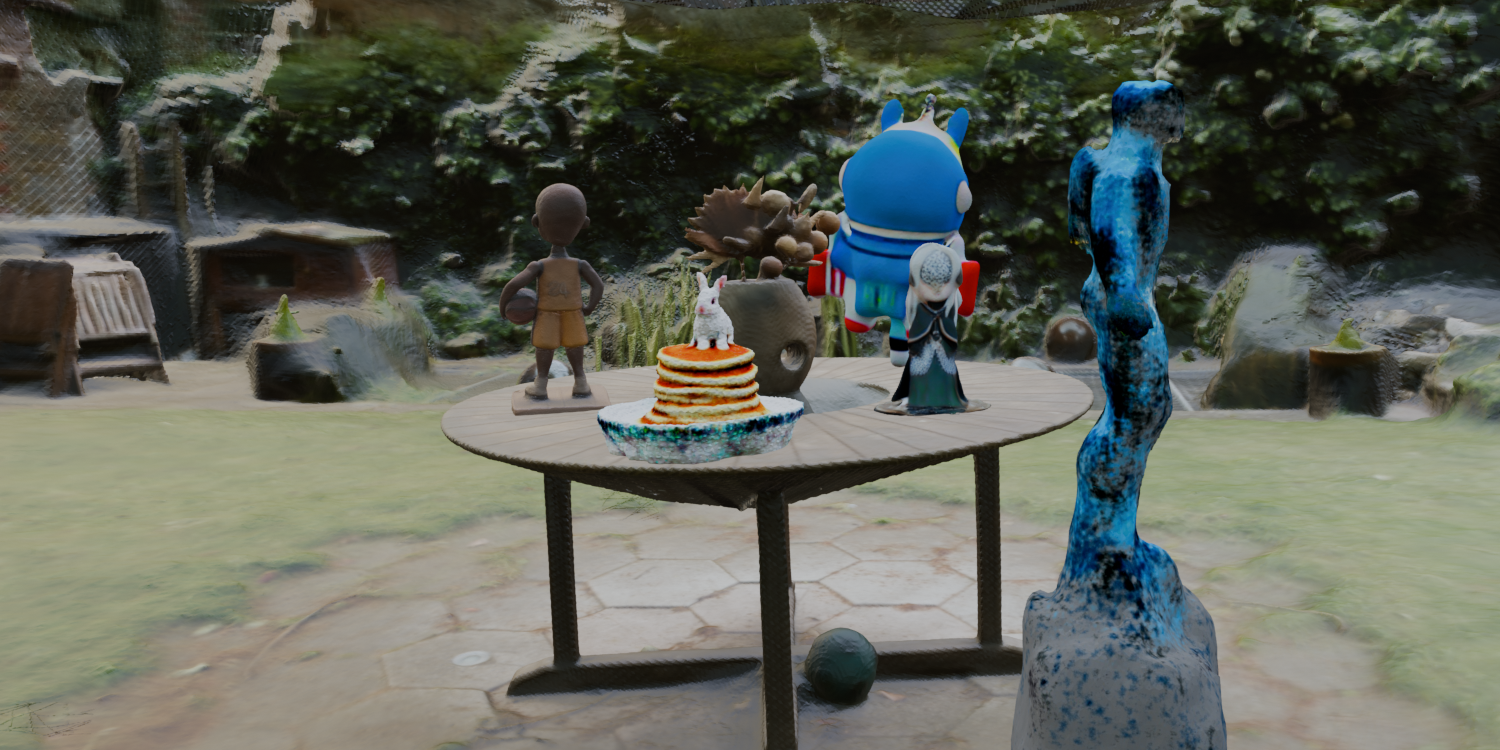
\includegraphics[width=\linewidth]{figures/task1/full_3.png}
	\end{minipage}
	\hfill
	\begin{minipage}{0.45\textwidth}
		\centering
		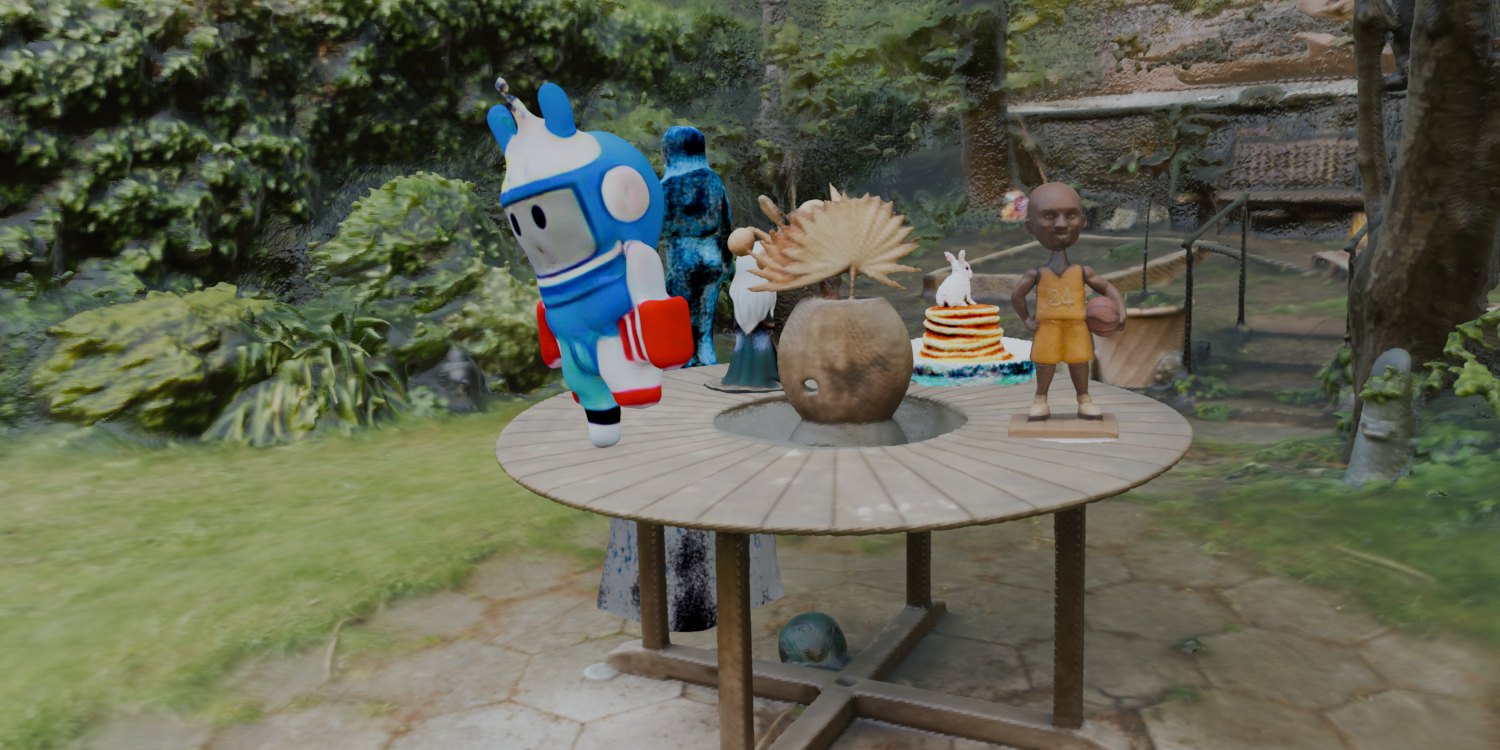
\includegraphics[width=\linewidth]{figures/task1/full_4.png}
	\end{minipage}
	
	\caption{Fusion Visualizations.}
	\label{fig:Fusion Vis}   % 原样保留（包括空格）
\end{figure}

Else, the rendered videos are provided in the appendix (see section~\ref{sec:models}).